\documentclass[10pt,twocolumn,letterpaper]{article}

\usepackage{cvpr}
\usepackage{times}
\usepackage{epsfig}
\usepackage{graphicx}
\usepackage{amsmath}
\usepackage{amssymb}
\usepackage[]{algorithm2e}

\usepackage{url}


% Include other packages here, before hyperref.
\usepackage[italian]{babel}
\usepackage[utf8x]{inputenc}
\usepackage{listings}
\usepackage{color}
\usepackage[dvipsnames]{xcolor}
% If you comment hyperref and then uncomment it, you should delete
% egpaper.aux before re-running latex.  (Or just hit 'q' on the first latex
% run, let it finish, and you should be clear).
\usepackage[pagebackref=true,breaklinks=true,letterpaper=true,colorlinks,bookmarks=false]{hyperref}

\cvprfinalcopy % *** Uncomment this line for the final submission

\def\cvprPaperID{****} % *** Enter the CVPR Paper ID here
\def\httilde{\mbox{\tt\raisebox{-.5ex}{\symbol{126}}}}

\newcommand{\Rplus}{\protect\hspace{-.1em}\protect\raisebox{.35ex}{\smaller{\smaller\textbf{+}}}}
\newcommand{\CC}{\mbox{C\Rplus\Rplus}\xspace}
\newcommand{\code}[1]{\texttt{#1}}

\definecolor{monokai@black}{HTML}{2C2C2A}
\definecolor{monokai@gray}{HTML}{524F52}
\definecolor{monokai@yellow}{HTML}{FDF5A9}
\definecolor{monokai@orange}{HTML}{FD971F}
\definecolor{monokai@red}{HTML}{DC322F}
\definecolor{monokai@magenta}{HTML}{D33682}
\definecolor{monokai@violet}{HTML}{F7208B}
\definecolor{monokai@blue}{HTML}{004C99}
\definecolor{monokai@green}{HTML}{009900}
\renewcommand{\lstlistingname}{Codice}
\lstdefinestyle{customC}{
frame=lines,
language=C++,
aboveskip=3mm,
belowskip=3mm,
showstringspaces=false,
columns=flexible,
basicstyle={\small\ttfamily},
numbers=left,
numberstyle=\tiny\color{monokai@black},
numbersep=5pt,
stepnumber=2,
breaklines=true,
tabsize=2,
numberstyle=\color{monokai@gray},
keywordstyle=\color{monokai@blue},
stringstyle=\color{monokai@green}\ttfamily,
identifierstyle=\color{monokai@black},
commentstyle=\color{monokai@blue},
emphstyle=\color{monokai@red},
otherkeywords={size_t}
    }

\ifcvprfinal\pagestyle{empty}\fi
\begin{document}

%%%%%%%%% TITLE
\title{Bigrams frequency counts using C++ threads}

\author{Filippo Mameli\\
filippo.mameli@stud.unifi.it
}

\maketitle
\thispagestyle{empty}

%%%%%%%%% ABSTRACT
\begin{abstract}
  Un bigramma (o digramma) è un gruppo di due lettere o parole consecutive.
  L'analisi della frequenza dei bigrammi è comunemente usata nella crittoanalisi o nell'apprendimento automatico.
  In questo documento si presenta un programma scritto in C++ che conta le occorrenze di bigrammi in un testo.
  Si mostrano inoltre le differenze di prestazioni tra il programma nella versione parallela e quella sequenziale.
  I principali strumenti utilizzati sono la classe std::Thread e la libreria Boost.
\end{abstract}

\noindent\large\textbf{Permessi di distribuzione}\\
\indent L'autore di questa relazione permette che questo documento possa essere distribuito a tutti gli studenti UNIFI dei corsi futuri.

\section{Introduzione}
Un bigramma è una sequenza di due lettere o parole addiacenti. I bigrammi sono utilizzati in vari ambiti.
L'analisi statistica del testo con i bigrammi è usata ad esempio in crittoanalisi, in apprendimento automatico o nel riconoscimento vocale.
Nella relazione si descrive un programma parallelo scritto in \CC che conta le frequenze dei bigrammi di lettere in un testo.
Nella sezione \ref{analisi} si mostrano inoltre le differenze prestazionali tra il programma parallelo e la sua controparte sequenziale, mostrando
lo Speedup e i tempi di esecuzione tra differenti documenti di testo.
Nel programma si utilizzano principalmente la classe della libreria standard Thread e la libreria Boost.
\vspace{3cm}

%-------------------------------------------------------------------------
\section{Algoritmo di base}
\label{algoritmobase}
Il programma deve parsare ogni singola parola e aggiornare il contatore dei bigrammi trovati.
La struttura dati per contare le occorrenze è l'Hashtable. Questa è stata scelta perché l'operazione più
usata è la ricerca del bigramma trovato e il conseguente incremento del contatore.
In un Hashtable l'operazione di ricerca ha complessità di tempo pari a $O(1)$ nel caso medio e per questa qualità,
la struttura è adatta per l'aggiornamento delle occorrenze.
Nell'algoritmo successivo vi è descritto in speudocodice i passaggi che sono effettuati.
\begin{algorithm}
  \caption{Algoritmo di base}
  \label{alg:algBase}
 \KwData{File di testo}
 \KwResult{Frequenza dei bigrammi contati}
 lettura del file di testo\;
 \While{fine del file non raggiunto}{
  \For{per ogni parola in file}{
   \For{per ogni bigramma nella parola}{
    Hashtable[bigramma]++\;
    }
   }
  }

\end{algorithm}


%-------------------------------------------------------------------------
\section{Parallelizzazione}
Dall'algoritmo di base si può ricavare facilmente una versione parallelizzata del programma.
Infatti è possibile dividere il file in più parti e assegnare ogni porzione ad un thread
che potrà eseguire il conteggio dei bigrammi solo sul singolo frammento.
Per far questo si deve suddividere il file e poi creare tanti thread quante sono le parti del documento.
Il problema principale è la struttura dati condivisa dai thread per aggiornare le occorrenze dei bigrammi.
Le strutture dati nella libreria standard di \CC non garantiscono il comportamento delle operazioni di modifica dei dati
da parte di più thread. Infatti se due o più thread devono aggiornare il contatore di un singolo bigramma, c'è un
problema di dipendenza nell'operazione di modifica.
Per questo motivo è stata creata una classe che ingloba \code{std::unordered\_map} e rende thread safe
le operazioni necessarie.
\subsection{Divisione dell'esecuzione}
Nel Codice~\ref{code:thread} si può vedere come viene effettuata la creazione dei thread. Ad ogni ciclo si
aggiunge un thread al vettore \code{threads}. Ai thread viene associata una funzione \code{countFunction} che prende come argomenti
\code{edge} e \code{bottom} che indicano la posizione del file su cui deve operare il thread.
Alla fine del ciclo si richiama la funzione di \code{join} per ogni thread appartente al vettore \code{threads} per terminare la loro esecuzione.

\lstinputlisting[firstnumber= 43,firstline = 43, lastline = 48, style = customC, caption = Creazione dei thread, label = {code:thread}]{../bigramPar.cpp}

La funzione \code{countFunction} controlla ogni singola parola contenuta nel vettore \code{words} cercando le sottostringhe di lunghezza 2 (Codice~\ref{code:count} linea 58).
Se il bigramma non è presente nell'hashMap (cioè \code{count(bigram)==0}), si inserisce.
Altrimenti si richiama la funzione \code{add} che incrementa il contatore di una unità.
\lstinputlisting[firstnumber= 55,firstline = 55, lastline = 64, style = customC, caption = Funzione del thread, label = {code:count}]{../bigramPar.cpp}

\subsection{Thread safe unordered map}
\code{threadsafe\_unordered\_map} è una classe wrapper di \code{std::unordered\_map}. In questa nuova classe la funzione di \code{insert} è thread safe e
\code{add} incrementa il valore del contatore dei bigrammi in modo atomico.
Come mostrato nel Codice~\ref{code:insert}, quando viene richiamata \code{insert} si utilizza \code{lock\_guard} per bloccare la struttura dati e garantire
il corretto funzionamento della funzione \code{countFunction}.
\lstinputlisting[firstnumber= 22,firstline = 22, lastline = 25, style = customC, caption = Funzione insert, label = {code:insert}]{../threadsafe_unordered_map.hpp}

L'atomicità della funzione \code{add} (Codice~\ref{code:add}) è data invece dall'uso di \code{atomic uint}. Utilizzando questa funzionalità di \CC non ci sono data race e si sincronizza
gli accessi all'hashmap tra i singoli thread.
\lstinputlisting[firstnumber= 13,firstline = 13, lastline = 20, style = customC, caption = atomic e Funzione add , label = {code:add}]{../threadsafe_unordered_map.hpp}

\subsection{Lettura del file e utilizzo del programma da terminale}
L'ultimo aspetto da trattare è la lettura del file e l'utilizzo del programma.
\code{ReadFileUtility} è la classe che legge il contenuto di un file (dato in input alla funzione \code{readInputFile}) e restituisce un vettore di parole.
In \code{readInputFile} si utilizzano le funzionalità della libreria Boost per la tokenizzazione delle parole nel testo.
Nel Codice~\ref{code:read} si può vedere che, passando il testo del file come stringa e \code{char\_separator} a \code{tokenizer}, si possa creare facilmente
il vettore \code{words} che verrà poi utilizzato per il conteggio dei bigrammi.
\lstinputlisting[firstnumber= 19,firstline = 19, lastline = 32, style = customC, caption = Read file, label = {code:read}]{../readFileUtility.cpp}

\subsubsection{Utilizzo del programma}
\label{util}
Da terminale si può utilizzare il programma specificando il percorso del file di testo e il numero thread che saranno creati. Si utilizzerà il numero di core della cpu
che la macchina ha a disposizione nel caso in cui non si indichi il numero di thread. Nel Codice~\ref{code:script} vi è un esempio.
\lstinputlisting[firstnumber= 1,firstline = 1, lastline = 2, style = customC, caption = Read file, label = {code:script}]{../scripts/par.sh}

\section{Analisi delle performance}
\label{analisi}
Per l'analisi delle performance sono stati utilizzati file di varie dimensioni. I tempi di esecuzione del programma parallelo
sono stati comparati con quelli della versione sequenziale. Quest'ultima non fa uso dei thread e utilizza \code{std::unordered\_map}
nella versione standard.

In Figura~\ref{fig:speed1} vi sono riportati gli Speedup rispetto alla scelta del file.
\begin{figure}
  \centering
    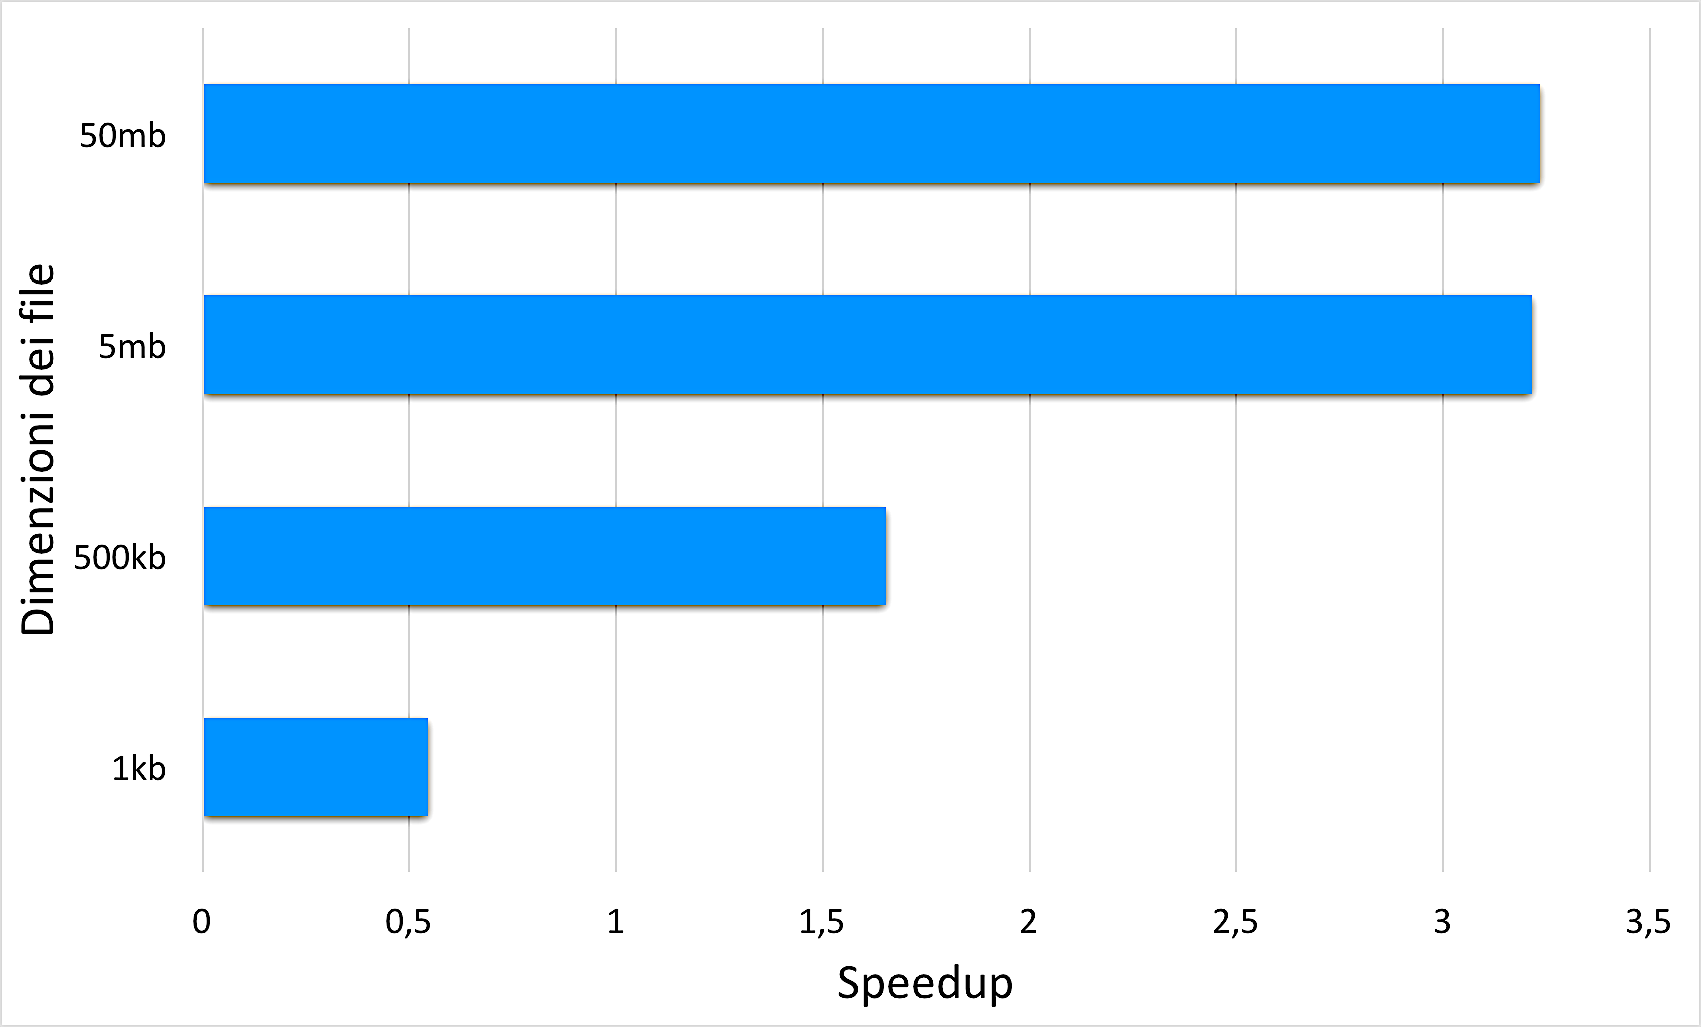
\includegraphics[width=\linewidth]{img/speed1.png}
  \caption{Speedup rispetto alle dimensione del file}
  \label{fig:speed1}
\end{figure}
I dati sono relativi al rapporto tra il tempo impiegato dal programma sequenziale e quello del programma parallelo che utilizza 4 thread(uno per ogni core della CPU).
Si può verdere che per file molto piccoli (1kb) la versione parallela appesantisce l'esecuzione, ma già per il file di 500kb
il programma ha uno Speedup pari a 1.7. Per file intorno ai 5mb o superiori l'overhead causato dalla creazione dei thread diventa irrilevante e lo Speedup si porta intorno a 3.2 e si stabilizza.

La Figura~\ref{fig:speed2} mostra invece lo Speedup rispetto ad un unico file di dimensione 5mb cambiando il numero di thread.\\
\begin{figure}
  \centering
    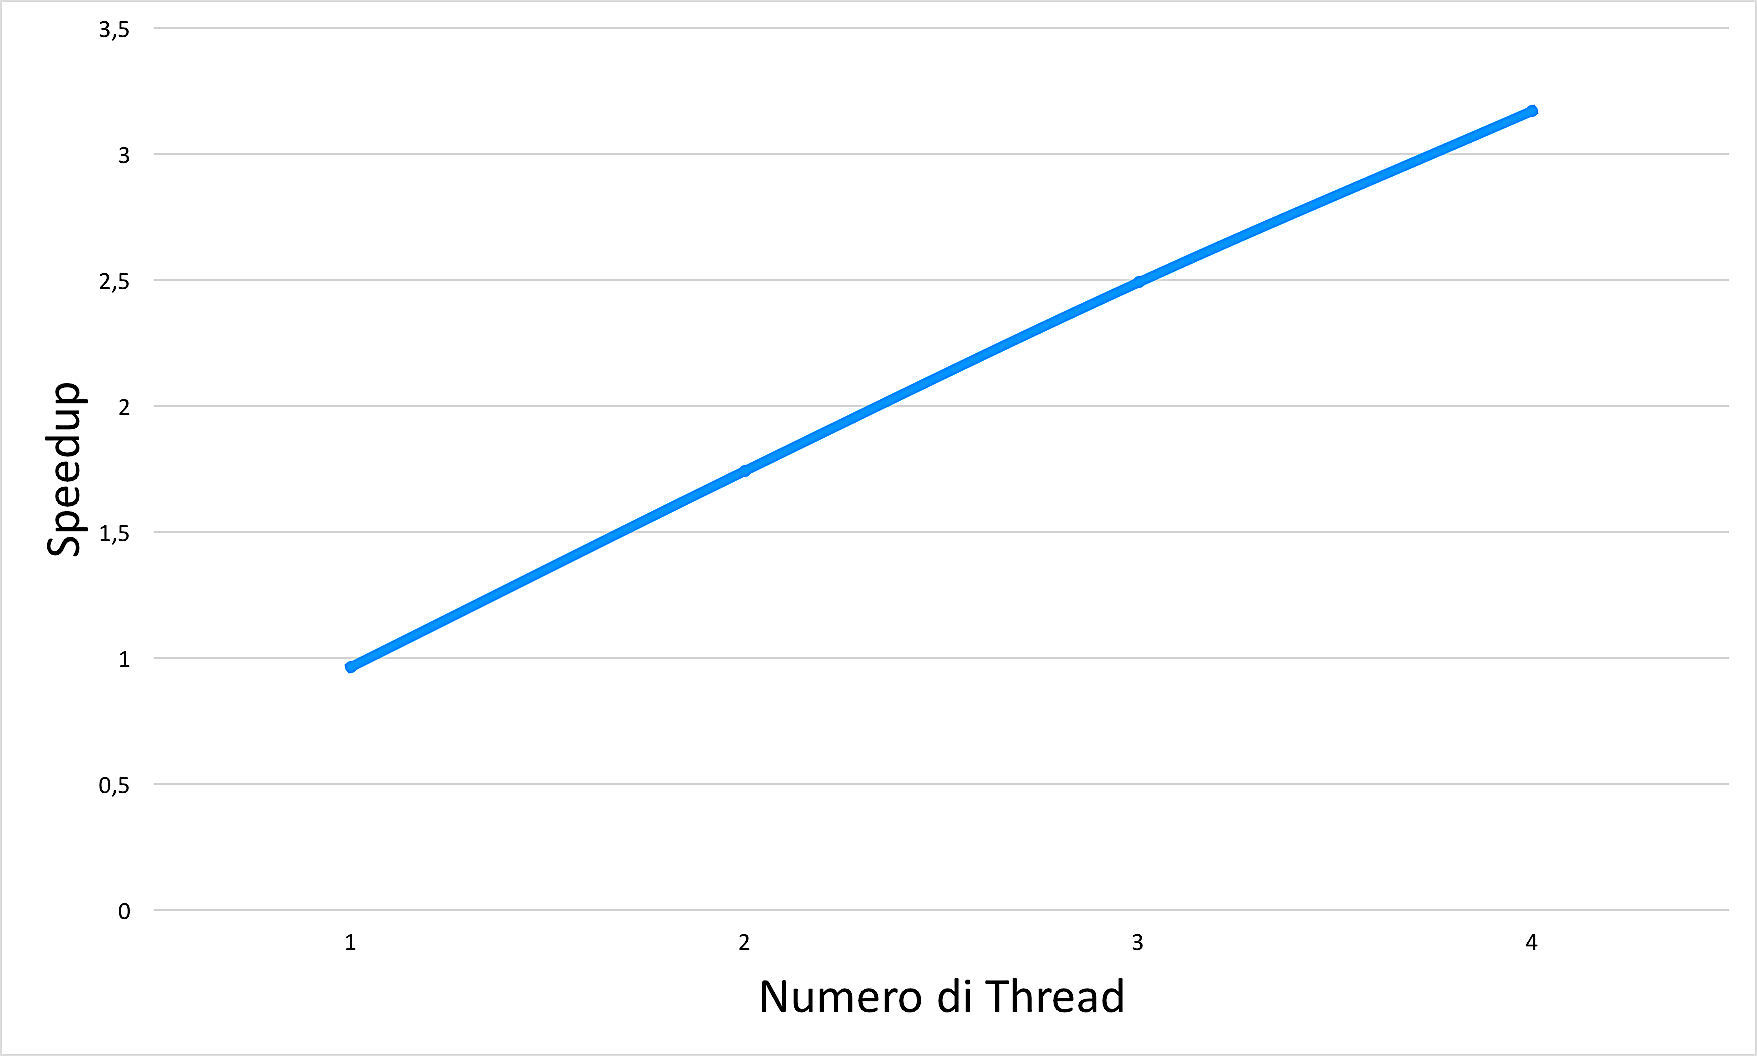
\includegraphics[width=\linewidth]{img/speed2.png}
  \caption{Speedup rispetto al numero di thread}
  \label{fig:speed2}
\end{figure}
In Figura~\ref{fig:ris} vi sono riportati i risultati assoluti in secondi. \\
\begin{figure}
  \centering
    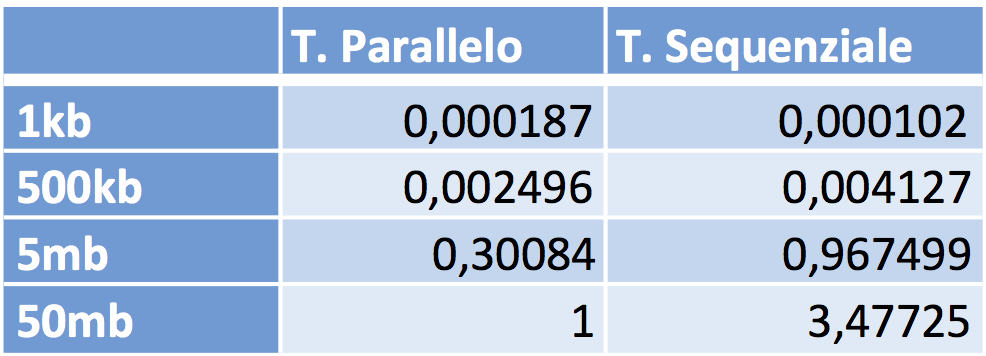
\includegraphics[width=\linewidth]{img/risultati.png}
  \caption{Speedup rispetto al numero di thread}
  \label{fig:ris}

  \end{document}
